\chapter{System Analysis}

\subsection{System Requirement Specification}

General structure of a user story described in this document: 
\\ \\
\begin{normalsize}
\textbf{\{User story name\}}: As a \{role\}, I want \{goal\}, so that \{benefit\} (\{priority\}).
\end{normalsize}

\subsection{Functional Requirements}
The following sections describe the data required and the functional requirements that shall be performed in the new ERP System for both the HQ and field-based staffs.  These functional requirements include the on-going System maintenance and the creation and management reports for all areas.

\begin{itemize}
	\item The System shall have a common database core which allows integration of data and transactions between all financial, operational, production, and customer service functions within the ERP System.
	\item The System shall have a graphic user interface (GUI) implemented  as a Web-based interface
	\item The System shall be able to export selected records into either pdf or table file format
	\item The System shall have administrator ERP System and user security functionality to include:
		\begin{itemize}
			\item Setting Up a New User
			\item Updating an Existing User
			\item Restricting User Access to Certain Roles
		\end{itemize}
	\item The System shall have the ability for generated reports to be savable and exportable to numerous devices and mediums including printers
	\item The System shall produce Fixed Asset Depreciation Schedules
\end{itemize}

\subsection{Non-functional Requirements}

\paragraph{Reliability}
Reliability is the probability that the System will be able to process work correctly and completely without being aborted.
\\
The proposed ERP System has varying degrees of impact on areas of Stadia should parts of the System fail.
If the Core Systems functional areas of the System fail (becomes unusable) for a period of time the impact on Stadia would be as follows:

\begin{center}
\begin{table}[!hb]
\begin{tabular}{ | m{10em} | m{25em}| } 
  \hline
  \textbf{Length of Time of Outage} & \textbf{Impact to Stadia} \\ 
  \hline
   One Hour & Some Impact to {{TODO}} \\ 
   \hline
   One Day & Medium to Large Impact {{TODO}} \\
   \hline
   One Week & Very Large to Catastrophic Impact. \\
  \hline
\end{tabular}
\caption{Impact of reliablity on Stadia}
\end{table}
\end{center}


\section{System Requirement Analysis}

\subsection{Actor and Use Case Identification}
A use case diagram is a graphic depiction of the interactions among the elements of a system. A use case is a methodology used in the system analysis to identify, clarify, and organize system requirements in this context, the term \"system" refers to something being developed or operated such as a mail-order product sales and service website. Use case diagram are employed in UML (Unified Modeling Language). A standard notation for the modeling of real-world object and systems. System objectives can include planning overall requirements validating a hardware design, testing and debugging a software product under development, creating an online help reference, or performing a consumer-service oriented task. For example, use case in a product sales environment would include item ordering, catalog updating payment processing, and customer relations. A use case diagram contains four components.

\begin{figure}[!h]
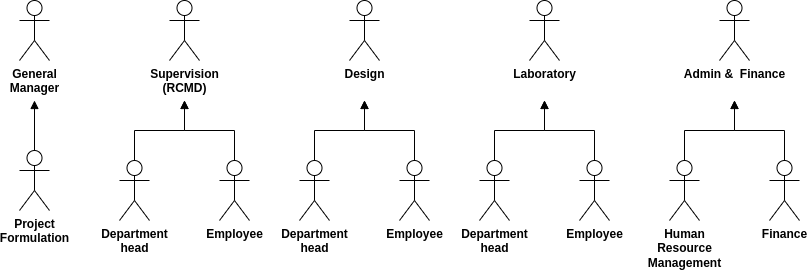
\includegraphics[width=13cm, keepaspectratio]{usecases/actors.png}
\label{shop_actors}
\caption{Actors involved }
\end{figure}

\subsection{Use Case Diagram}

Use case diagrams are used during the analysis
process to find system requirements and to design
system functionality. In this study use case
diagrams are used to describe the access rights of
each actor. Administrator Actors generally have a
function to manage users such as creating accounts
and setting access rights.

\subsubsection{Administrator Use Case Diagram}

\subsubsection{Manager Use Case Diagram}

\subsubsection{HR Use Case Diagram}

\subsection{Activity Diagram}

\subsubsection{Recruitment Module Activity Diagram}

\subsubsection{Human Resources Activity Diagram}

\subsubsection{Attendance Activity Diagram}

\subsubsection{Leave (time off) Activity Diagram}

\subsubsection{Payroll Activity Diagram}

\subsubsection{Performance Management (Appraisal) Activity Diagram}

\subsubsection{Asset Management Activity Diagram}


\subsection{User Access Rights}

\hspace{-2cm}
\begin{tabularx}{540pt}{|X|c|c|c|c|c|c|c|p{3cm}|}

%{|*{9}{Y|}}

\hline

\textbf{No} & \textbf{User} & \textbf{Acess Level} & \textbf{Object} & \multicolumn{4}{c|}{\textbf{Acess Right}} & \textbf{Information} \\
\cline{5-8} & &  &  & Read & Write & Create & Delete & \\

\hline

\multirow{1}{*}{1} & \multirow{1}{*}{Administrator} & \multirow{1}{*}{Administration} & ALL & \cmark & \cmark & \cmark & \cmark & Top Level \\

\hline

\multirow{2}{*}{2} & \multirow{2}{*}{System Admin} & \multirow{2}{*}{System Admin} & 
User & \cmark & \cmark & \cmark & \xmark & Second level below Administrator \\
\cline{4-8} & & & 
Acess Right 2 & \xmark & \xmark & \xmark & \xmark & \\

\hline

\multirow{2}{*}{3} & \multirow{2}{*}{Manager} & \multirow{2}{*}{Manger} & 
Attendance & \cmark & \cmark & \xmark & \xmark & Manager \\
\cline{4-8} & & & 
Acess Right 2 & \xmark & \xmark & \xmark & \xmark & \\

\hline

\end{tabularx}
\hspace*{-1cm}

